\documentclass[12pt, letterpaper]{article}
\usepackage{multicol}
\usepackage{natbib}
\usepackage{titling}
\usepackage{graphicx}
\graphicspath{{images/}}
\usepackage[toc,page]{appendix}
\usepackage{subcaption}
\setlength{\columnsep}{0.6cm}
\usepackage[margin=1.2in]{geometry}
\title{Wall-Following with a LEGO Robot}
\author{William Ewart}
\date{March 2017}

\begin{document}
\begin{titlingpage}
\maketitle
\tableofcontents
\end{titlingpage}
\newpage

\begin{multicols}{2}
\section{Introduction}
In this paper with Rowan Walshe and David Lambeth we created a LEGO robot to navigate a room using an EV3 brick running ev3dev. We hypothesised that the time it takes the robot to move around the room and the number of bumps that the robot does while doing this will be influenced by the speed. Our motivation for making a reactive robot came from \cite{Brooks} paper on intelligence without representation. The hypothesis was thought of during the testing of the robot, when we discovered that varying speeds affected the manner in which the robot navigated the test course and the number of bumps made with the edges of the test  course. We found that as the speed of the robot increased the time taken to finish navigating the room decreased up to a point and the number of bumps also increased with it. 
\section{Approach}
The robot uses a finite state machine to react to the environment in different ways. The robot was developed this way as \cite{Bryson} states that a finite state machine is the standard way of controlling agents. The transitions between states is also not complex enough that we needed to use a different method. The robot will change states depending on the readings from its sensors. One difficulty we came across during development was noisy readings from the ultrasonic sensor. To overcome this we took an average of the last three readings to smooth out any noise that may occur. Another issue we found when the robot was when it was turning to get closer to a wall or around a corner. Due to the ultrasonic sensor being fixed, if the robot turned too sharply the wall got further away relative to the ultrasonic sensor. This would then cause the robot to keep turning towards the wall. To correct this we made the robot move forwards so that the sensor would get closer to the wall, correct itself and then continue as normal. A picture of the robot can be seen in appendix \ref{Robot} that shows its sensor configuration.
The room used was for the experiment was different to the one that the robot used while it was being tested. This ensures that there were no hard coded behaviours into the robot to just deal with the experiment room. The room contained a few obstacles that were put there by us to challenge it a bit more and to see how it would react to those obstacles.
The robot performed three runs at varying speeds with the time to navigate the room and the number of bumps being recorded, an average of these results was subsequently taken. During the experiment we found that the bumper sensors did not always activate as they should. We speculated that this was due to the design of the bumper. This caused a few interventions and at later speeds the bumper was coming off causing failed runs. This issue prevented us testing the maximum speeds of the robot.
\section{Results}
The average time for the robot to complete the course decreased as the speed of the robot increased. At the slowest speed tested the robot completed the course in an average time of 210 seconds with a standard deviation of 5.998. At half speed the robot completed the course in an average of 106 seconds with a standard deviation of 2.815. At the highest speed tested the robot completed the course in an average time of 88 seconds with a standard deviation of 3.71. 
The graph plotted for this can be seen in appendix \ref{Time}. 

\begin{center}
	\begin{tabular}{ |c|c|c|c| } 
		\hline
		Speed & Time (seconds) & Std Dev \\ \hline
		0.2 & 210 & 5.998\\ \hline
		0.3 & 154 & 6.004\\ \hline
		0.4 & 124 & 3.015\\ \hline
		0.5 & 106 & 2.815\\ \hline
		0.6 & 90  & 4.039\\ \hline
		0.7 & 88  & 3.71\\ \hline
	\end{tabular}
\end{center}

The average number of bumps increased when the speed of the robot increased. At the slowest speed the average number of bumps that the robot made was 23 with a standard deviation of 2. At half the maximum speed the amount of bumps made by the robot was 29 with a standard deviation of 1.527. At the maximum speed the average number of bumps was 32 with a standard deviation of 3.464. The graph for these results can be seen in appendix \ref{Bumps}.

\begin{center}
	\begin{tabular}{ |c|c|c|c| } 
		\hline
		Speed & Average Bumps & Std Dev \\ \hline
		0.2 & 23 & 2\\ \hline
		0.3 & 25 & 1.154\\ \hline
		0.4 & 24 & 1\\ \hline
		0.5 & 29 & 1.527\\ \hline
		0.6 & 27  & 2.081\\ \hline
		0.7 & 32  & 3.464\\ \hline
	\end{tabular}
\end{center}

\section{Discussion}
The results support that as the speed of the robot increases the time decreases to a point and the number of bumps increase. As the robot approaches maximum speed the decrease in average time starts to level off hinting that at faster speeds the time won't decrease and it could in fact increase. This is the same for the number of bumps where the results show an upward trend when the speed of the robot is increasing. However with the number of bumps it doesn't level off at the top suggesting that there will be more bumps as the speed increases. This could cause the robot to complete the course in more time as more bumps 
mean it will have to back up from the object more and thus taking more time. However as the robot is bumping more it may not get stuck in as many places as a slower robot could. This is something that could be explored in more depth. There were some speeds where less bumps happened even though the speed had increased. This could be due to a lack of data so more results for these speeds should be taken to see if they average out to what would be expected. Higher speeds should be tested to confirm the trend for the speed and bumps that was uncovered. Variable speeds around the room could also be tested to see if there is any differences when going slower around corners and faster on straights.
\section{Conclusion}
In conclusion we set about to create a reactive robot that could navigate around a room. We tested to see if the speed of the robot would effect the number of bumps off of objects and if there was a limit to the amount of time it would take to go around the room. We found that the number of bumps increased with speed and the time taken decreased up to a point. 
\newpage
\end{multicols}
\bibliographystyle{agsm}
\bibliography{bibliography}
\begin{appendices}
\section{Average time graph}
\label{Time}
\begin{figure}[!h]
\centering
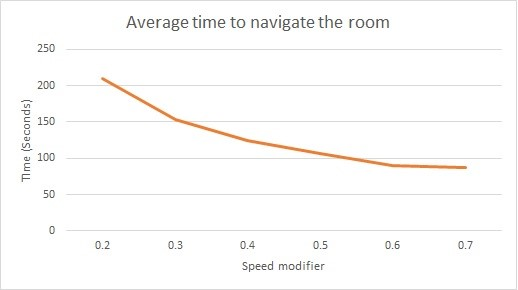
\includegraphics[width=\textwidth]{Timegraph}
\caption{Graph of the average time for the robot to navigate the room at different speeds}
\end{figure}
\newpage
\section{Average bumps graph}
\label{Bumps}
\begin{figure}[!h]
\centering
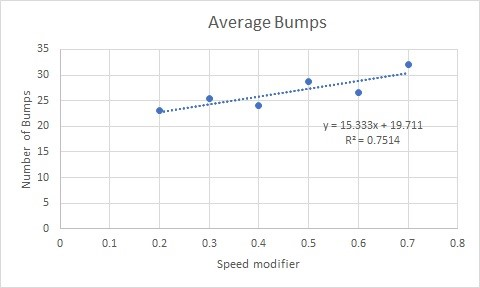
\includegraphics[width=\textwidth]{Bumpgraph}
\caption{Graph of the average time for the robot to navigate the room at different speeds}
\end{figure}

\section{Robot Picture}
\label{Robot}
\begin{figure}[!h]
\centering
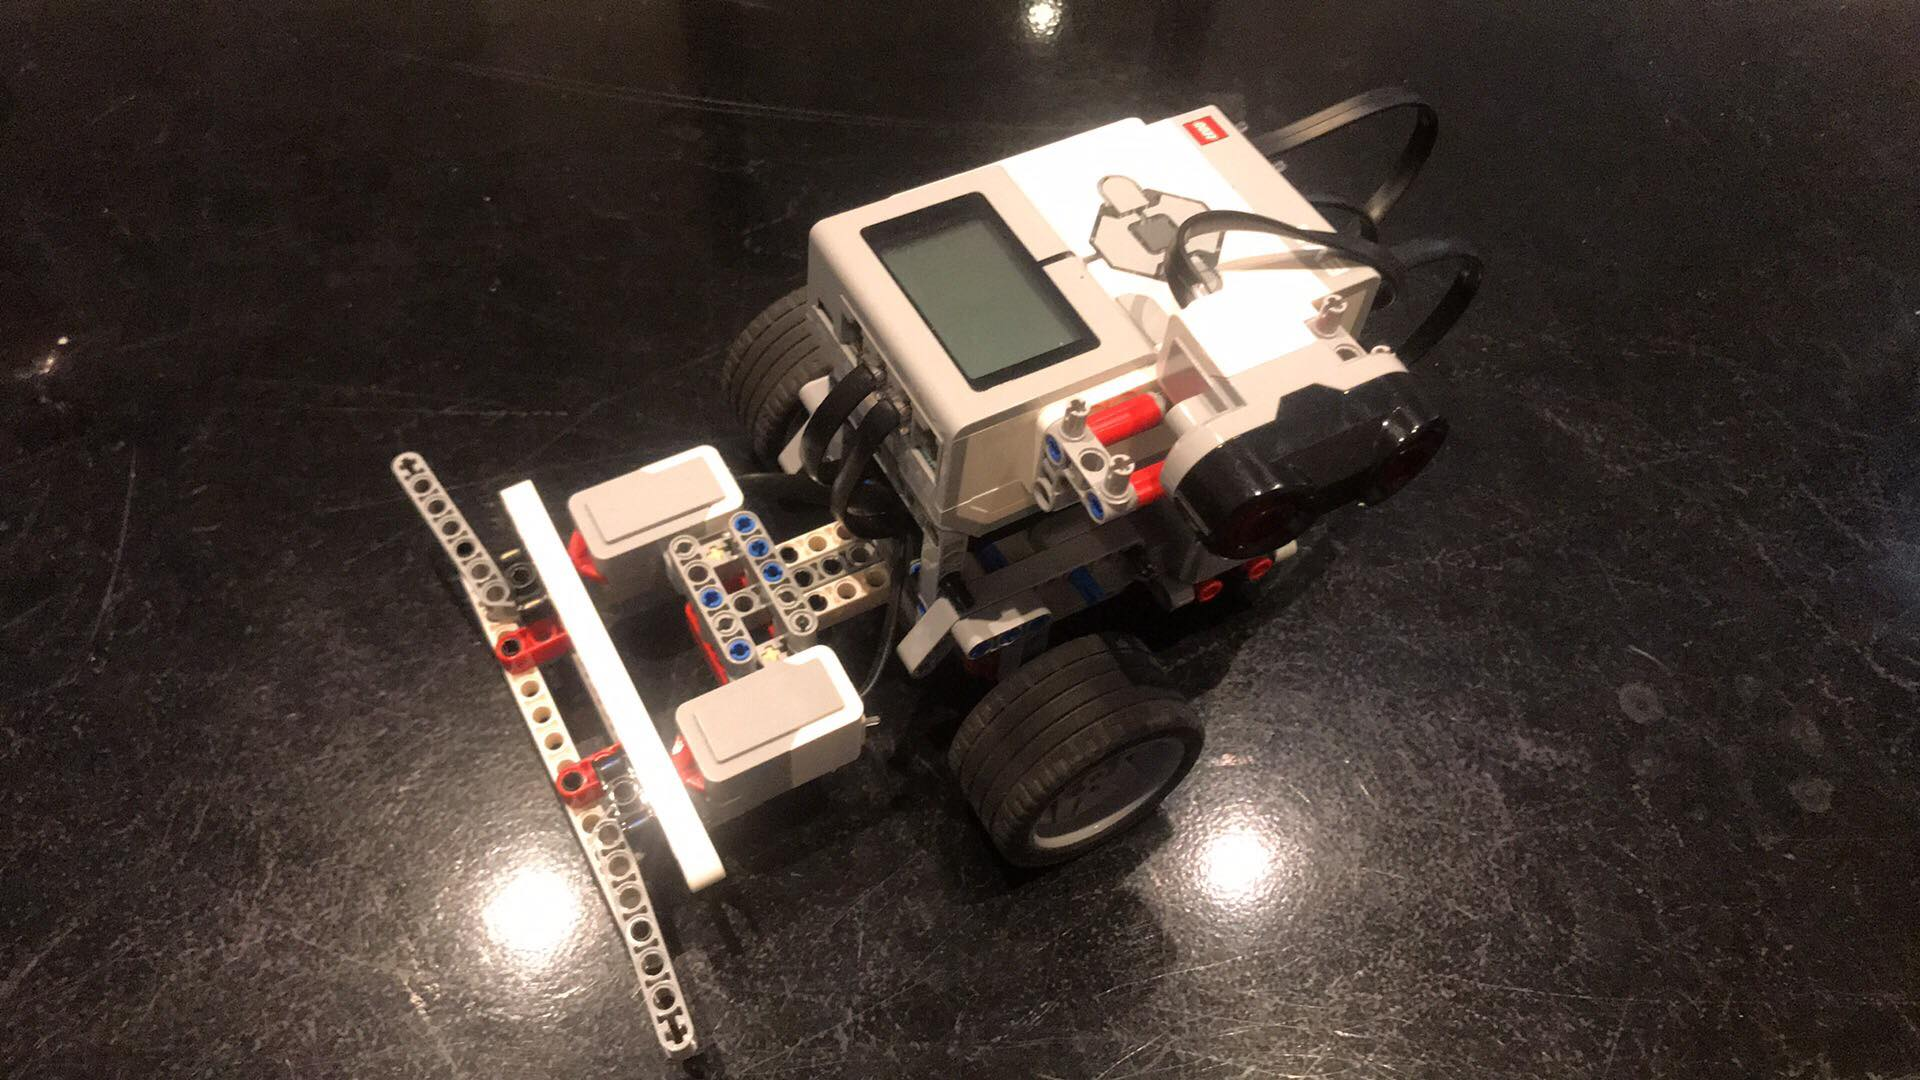
\includegraphics[width=0.5\textwidth]{Robot}
\caption{Picture of the final robot design}
\end{figure}
\end{appendices}

\end{document}